% Editorially assembled from the preserved September 17 report.
\section{Experimental validation}\label{sec:experiments}
The following findings concern the recorded frozen experiments, not universal optimality or safety claims. All detailed protocols and archived outputs are mapped in the accompanying source package~\cite{project2026}.
\subsection{Why the bridge preferred one extra column}\label{exp:E1}
The frozen rank-deficient bridge used $d=500$, $k\in\{5,15,30\}$, $\eta\in\{0,10^{-14},10^{-10},10^{-6}\}$, budgets $m\in\{80,160,240\}$, and 200 paths per setup. Matrix-orientation seeds were 52000--52002, one per rank and reused across tail levels; basis seeds were 70000--70199. Range sketches were nested coordinate-Rademacher prefixes. The frozen rank-aware QR used relative tolerance $10^{-12}$ and absolute tolerance zero, relative to its sampled-column reference scale---not a universal eigenvalue threshold.


The allocation grids ended at 36, 76, and 116 for the respective budgets, retaining a residual floor of eight in the full-rank planning grid. There were 554,400 trial-allocation rows. At $\eta=10^{-6}$, \textbf{all 138,600 individual rows} satisfied $r_q=q$, not merely an average-rank statement.


Here $q_X^\star$ denotes the chosen minimizer of the finite empirical mean risk curve on the tested allocation grid, using the frozen plateau/tie convention; it is not an individual path's minimizer or the unknown population optimum. In all nine rank--budget combinations at that tail level, the recorded minima were


\begin{equation}
q_{\rm rank}^\star=k,\qquad q_G^\star=q_R^\star=k+1.
\end{equation}


At $m=160$, the reproduced means were:


{\small
\begin{longtable}{@{}>{\raggedright\arraybackslash}p{0.1408\linewidth}>{\raggedright\arraybackslash}p{0.1848\linewidth}>{\raggedright\arraybackslash}p{0.1848\linewidth}>{\raggedright\arraybackslash}p{0.1848\linewidth}>{\raggedright\arraybackslash}p{0.1848\linewidth}@{}}
\caption{Mean conditional risks at the knee (budget 160)}\label{tab:auto2}\\
\toprule
$k$ & Gaussian risk at $k$ & Gaussian risk at $k+1$ & Rademacher risk at $k$ & Rademacher risk at $k+1$ \\
\midrule
\endfirsthead
\toprule
$k$ & Gaussian risk at $k$ & Gaussian risk at $k+1$ & Rademacher risk at $k$ & Rademacher risk at $k+1$ \\
\midrule
\endhead
5 & $6.5616\times10^{-11}$ & $6.6759\times10^{-12}$ & $5.8695\times10^{-11}$ & $7.9857\times10^{-14}$ \\
15 & $1.2123\times10^{-8}$ & $7.5641\times10^{-12}$ & $1.2059\times10^{-8}$ & $2.4140\times10^{-13}$ \\
30 & $1.5521\times10^{-11}$ & $9.5731\times10^{-12}$ & $6.5597\times10^{-12}$ & $5.9134\times10^{-13}$ \\
\bottomrule
\end{longtable}
}
The denominator thresholds $(D-2)/D$ are respectively $148/150$, $128/130$, and $98/100$. They require energy reductions of only $1.3333\%$, $1.5385\%$, and $2\%$. To compare means correctly, multiply each mean-risk ratio by $(D-2)/D$ to obtain the corresponding ratio of mean energies. The large reductions in the table are not explained by the denominator; the denominator penalizes the extra direction.


The mechanism audit~\cite{project2026} connected poorly conditioned near-square signal blocks, principal-angle errors, and tail-dominated conditional risk along nested paths. However, median behavior often preferred $k$, Gaussian bootstrap intervals for the mean difference at $m=160$ included zero, and sensitivity experiments produced shifts of zero, one, two, or more. Rare one- or two-path failures can dominate a finite mean. The strongest conclusion is therefore \textbf{modest oversampling can protect against rare capture failures; exactly one extra column is not a universal optimum}.

\subsection{Fresh probes contain a useful signal, not a theorem}\label{exp:E2}
The offline risk-discrimination experiment reconstructed 200 frozen paths for each of three ranks and two tail levels. Each path received four batches of 50 certification repetitions with nested $s\in\{4,8,16,32\}$. The same fresh probes served all actions, budgets, estimators, and both tail levels, so these comparisons are paired.


The estimators were ordinary sample variance, the independent-pair mean, and two medians of block means. For $W_j=(X_{2j-1}-X_{2j})^2/2$, $\mathbb EW_j=\sigma^2$; the sample variance and pair mean are unbiased families. \texttt{mom\_w1} takes the median of individual $W_j$ values; \texttt{mom\_w2} takes the median of two-$W$ block means. At $s=16$ they have eight and four blocks. Neither is generally unbiased. At $s=4$ both coincide with the pair mean, and at $s=8$ \texttt{mom\_w2} does too; these degeneracies are not independent evidence.


The primary comparison was $q=k+1$ against $q=k$ at $m=160$, $\eta=10^{-6}$, $s=16$. The empirical guard used $\varepsilon=1/3$, so acceptance required an estimated candidate risk no more than half the estimated baseline risk. Rejection used the reverse ratio; equality or insufficient separation meant abstention. No finite-sample confidence event was attached to this rule.


{\small
\begin{longtable}{@{}>{\raggedright\arraybackslash}p{0.4224\linewidth}>{\raggedright\arraybackslash}p{0.1936\linewidth}>{\raggedright\arraybackslash}p{0.2640\linewidth}@{}}
\caption{Primary sample-variance operating rates (16 certification probes)}\label{tab:auto3}\\
\toprule
Sample-variance primary metric & Point estimate & Conditional 95\% bootstrap interval \\
\midrule
\endfirsthead
\toprule
Sample-variance primary metric & Point estimate & Conditional 95\% bootstrap interval \\
\midrule
\endhead
False-safe rate among truly worse paths & 0.0134\% & [0.0028\%, 0.0305\%] \\
False-rejection rate among truly better paths & 0.5157\% & [0.2991\%, 0.7722\%] \\
Top-5\% true-better catastrophic detection & 79.6667\% & [69.0662\%, 89.2833\%] \\
Acceptance among all truly better paths & 52.0991\% & [40.3055\%, 63.5069\%] \\
\bottomrule
\end{longtable}
}
Rates average repetitions within each frozen path, eligible paths within rank, then ranks equally. False-safe denominators contain only truly worse paths; false-rejection denominators only truly better paths. Catastrophic sets are defined within rank from the exact baseline risk and restricted to truly better primary candidates. The 10,000-replicate bootstrap resamples eligible path clusters within rank, not individual repetitions. Empty required rank populations are unevaluable rather than silently discarded. Truth ties and undefined zero-risk relative errors are treated separately.


The benign $\eta=10^{-10}$ control false-safe estimate was 0.0008\%, with interval [0\%, 0.0025\%]. The two MoM false-safe estimates were 4.6971\% and 1.5478\%, compared with 0.0134\% for sample variance. The independent-pair mean served as an ablation. These are empirical operating rates, not confidence guarantees for accepted actions.


\begin{figure}[tbp]
\centering
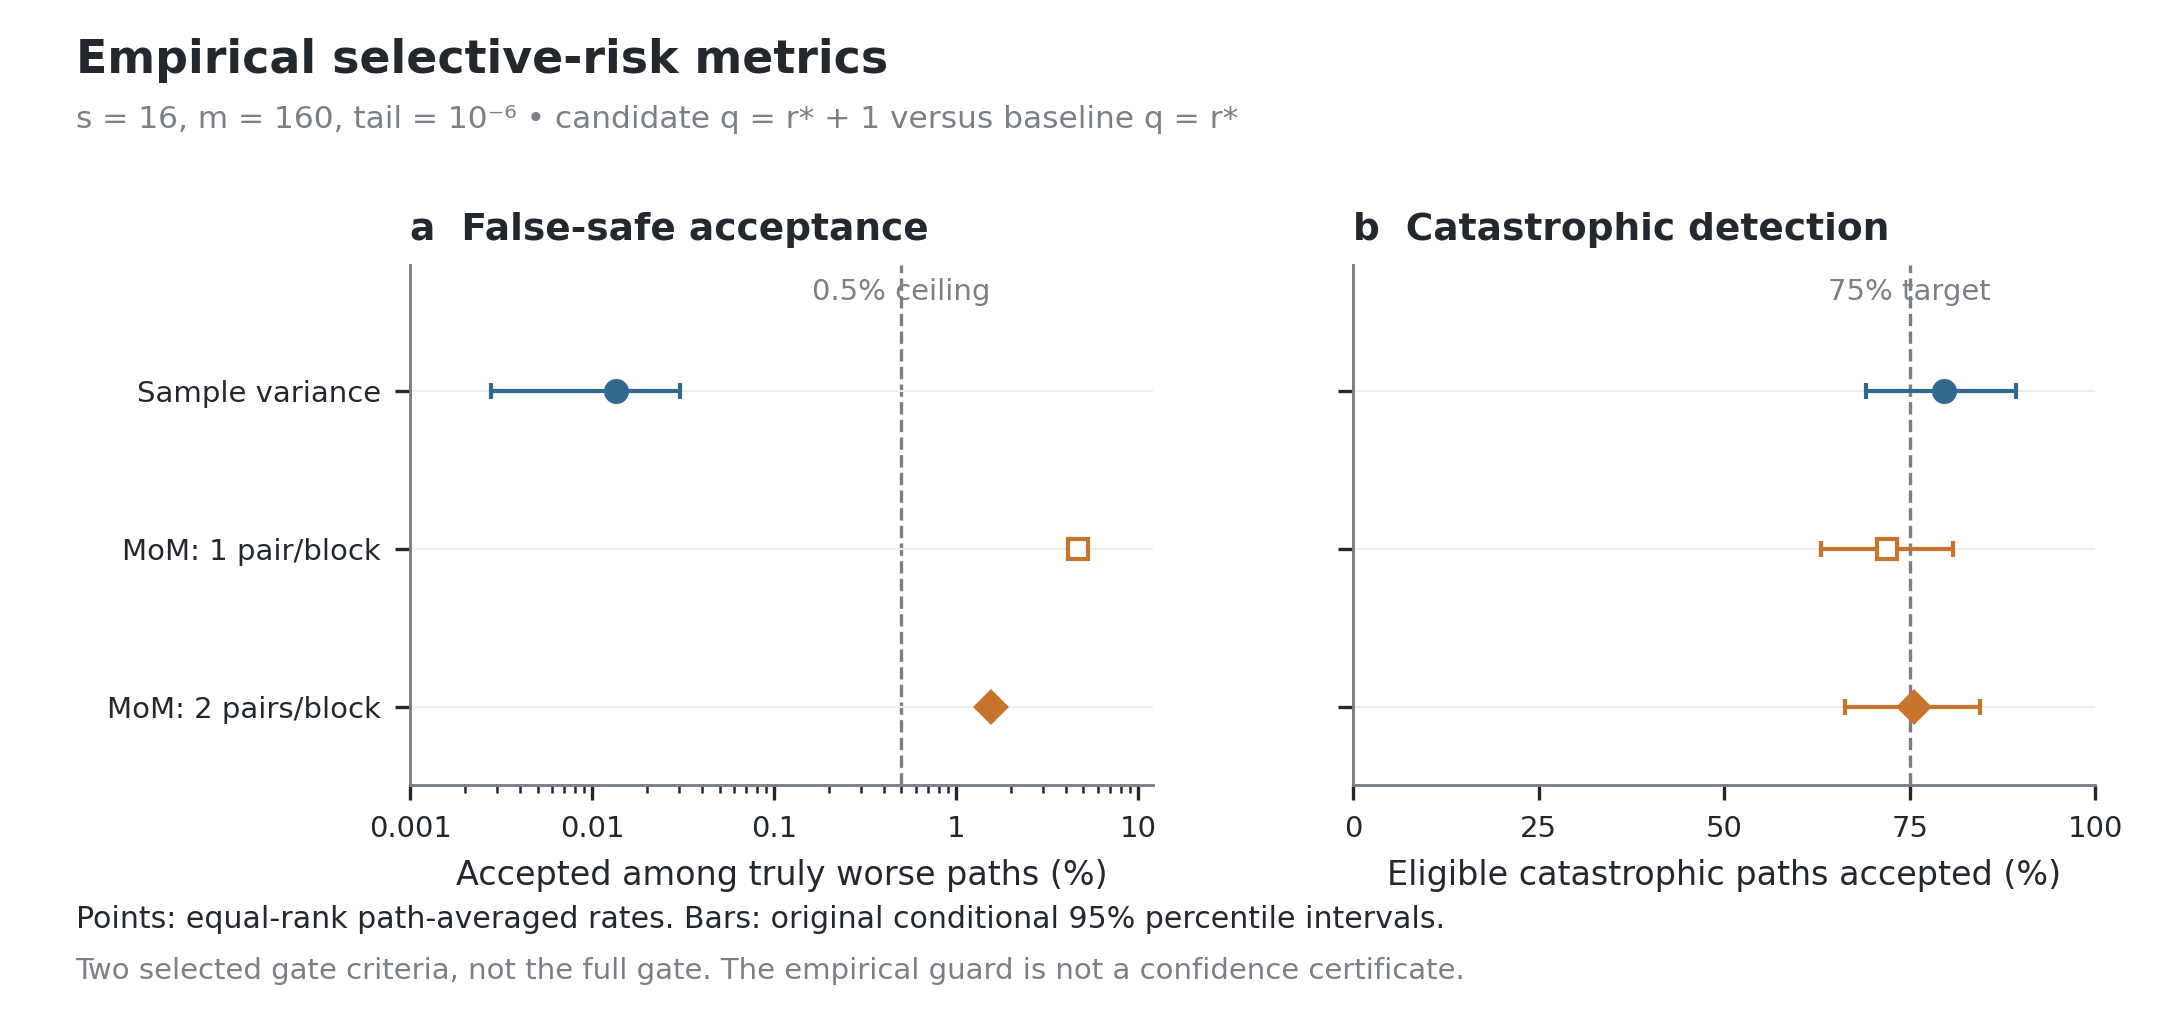
\includegraphics[width=\linewidth]{figures/figure2_empirical_signal.png}
\caption[Empirical direct-risk discrimination]{\textbf{Empirical direct-risk discrimination.} At $m=160$, $\eta=10^{-6}$, and $s=16$, compare $q=k+1$ with $q=k$ using the factor-two empirical guard. (a) Acceptance among truly worse paths. (b) Acceptance among true-better paths in the within-rank top 5\% of baseline risk. There are 200 paths per rank and 200 repetitions per path. Points average repetitions, eligible paths, then ranks equally. Bars are 95\% percentile intervals from 10,000 eligible-path, rank-stratified bootstrap replicates. Dashed lines show the selected descriptive thresholds, not confidence guarantees.}
\label{fig:signal}
\end{figure}
\subsection{Paying for certification changed the conclusion}\label{exp:E3}
The budget-charged emulation deducted construction and certification costs before final estimation. Across 600 frozen paths, the equal-rank average of within-rank \textbf{ratios of mean risks} was 0.036329, with conditional bootstrap interval [0.014628, 0.639830]. The paid oracle was 0.035411 and the paid fallback 1.172197.


Nevertheless, \textbf{575 of 600 individual paths---95.83\%---were harmed} relative to their original baseline. The pooled median pathwise ratio was 1.160714. The historical value 1.172197 described an equal-rank average of within-rank medians in the relevant summary, not that pooled median. Means of ratios, ratios of means, and averages of medians are distinct statistics.


\begin{figure}[tbp]
\centering
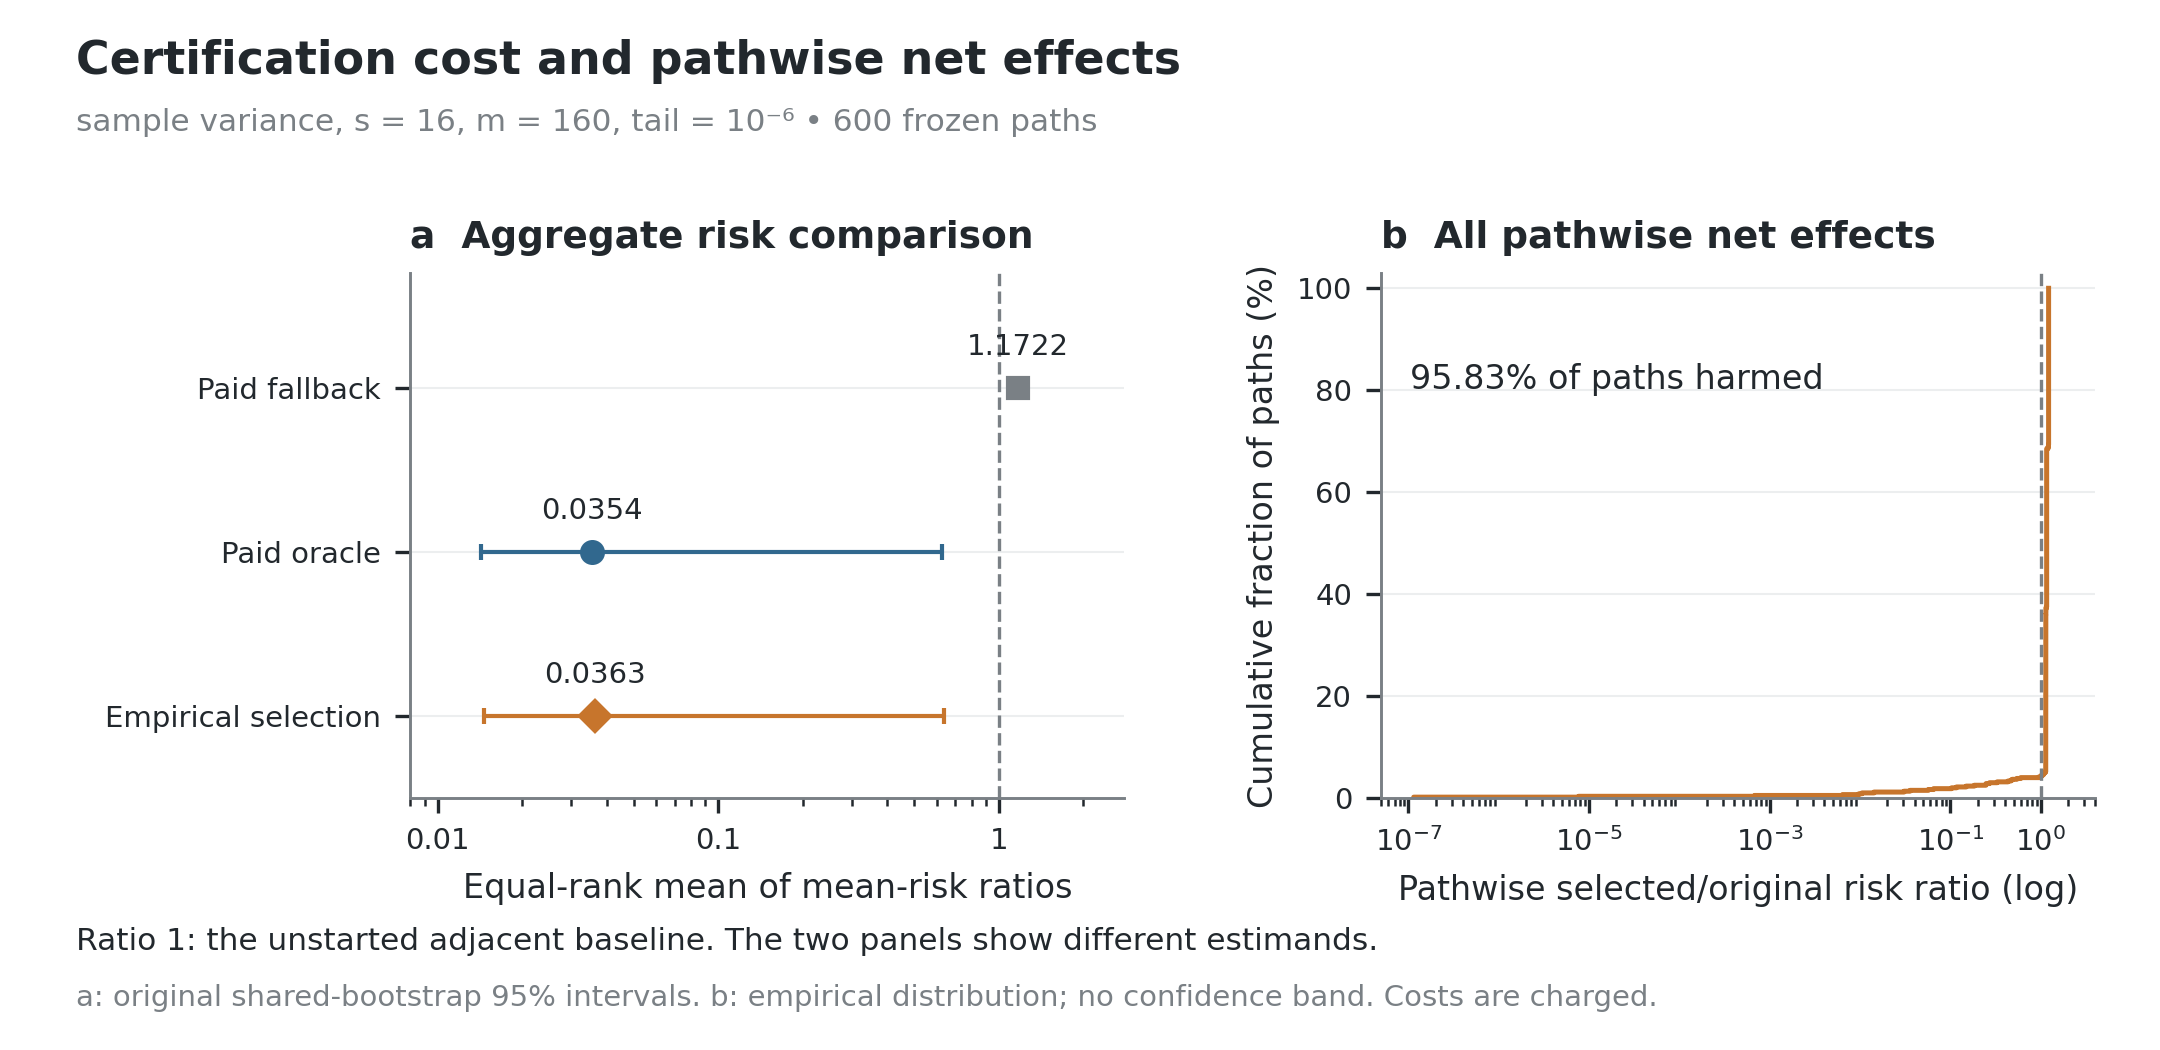
\includegraphics[width=\linewidth]{figures/figure3_certification_cost.png}
\caption[Certification cost and rare-path protection]{\textbf{Certification cost and rare-path protection.} The same 600 paths use sample variance with $s=16$, $m=160$, and $\eta=10^{-6}$. The reference is the unstarted adjacent baseline. (a) Equal-rank averages of within-rank mean-risk ratios, with 95\% percentile intervals from 10,000 shared rank-stratified path-bootstrap replicates. The paid oracle uses exact offline risk; paid fallback always returns to the baseline basis after costs. (b) All 600 pathwise selection/original risk ratios, with no confidence band. Protecting rare costly baselines improves the aggregate mean despite increasing risk on most paths.}
\label{fig:cost}
\end{figure}
\subsection{Common-probe cancellation was strong on average, weaker on catastrophes}\label{exp:E4}
The common-probe comparison gave an equal-rank empirical paired/independent variance ratio of \textbf{0.151032}, with interval \textbf{[0.137069, 0.166735]}, approximately 84.9\% lower. The independent benchmark is the plug-in sum of marginal variances. Catastrophic paths had mean pairing ratio \textbf{0.899565}, compared with \textbf{0.111635} for ordinary paths. Thus the strongest cancellation did not occur on the rare paths most relevant to aggregate risk~\cite{project2026}.


\subsection{A sharp pilot knee missed an entire dominant direction}\label{exp:E5}
The recovered orientation experiment used $d=100,m=60$, six spectra, 30 Haar orientations plus a coordinate orientation, and ten paths per orientation. The heuristic first built an eight-column Rademacher pilot and cached its basis products. Among positive Ritz values exceeding $10^{-12}\theta_1$, it required at least four values and selected the largest adjacent logarithmic gap. If that gap was at least $1.5$, it used $q=\min(q_{\max},\max(8,j_{\rm gap}+2))$; otherwise it used $q_0=\min(q_{\max},\lfloor m/3\rfloor)$, where $q_{\max}=\min(d,\lfloor(m-2)/2\rfloor)$. Pilot products were reused, and fresh residual probes were Rademacher. No contrast filter was active.

For the rank-five step spectrum with $\eta=0.001$, every gate triggered and selected $(q,r,\ell)=(8,8,44)$. Standard Hutch++ used $(20,20,20)$. The finite observed comparison was:


{\small
\begin{longtable}{@{}>{\raggedright\arraybackslash}p{0.1408\linewidth}>{\raggedright\arraybackslash}p{0.1848\linewidth}>{\raggedright\arraybackslash}p{0.1848\linewidth}>{\raggedright\arraybackslash}p{0.1848\linewidth}>{\raggedright\arraybackslash}p{0.1848\linewidth}@{}}
\caption{Recovered rank-five step experiment}\label{tab:auto4}\\
\toprule
Orientation group & Paths & Gated MSE & Standard MSE & Gated / Standard \\
\midrule
\endfirsthead
\toprule
Orientation group & Paths & Gated MSE & Standard MSE & Gated / Standard \\
\midrule
\endhead
Haar orientations & 300 & $2.839433\times10^{-7}$ & $1.672813\times10^{-6}$ & 0.169740 \\
Coordinate aligned & 10 & $3.303942\times10^{-3}$ & $7.209998\times10^{-7}$ & 4582.446 \\
\bottomrule
\end{longtable}
}
The coordinate result is not erased by the rotated gain. Coordinate-Rademacher sketches are not rotation invariant, and the exact Rademacher residual risk depends on coordinates too.


In the seed-2026 replay, rows three and four of the failing signal block are exact negatives. Rational elimination verifies rank four. Therefore $w=(e_3+e_4)/\sqrt2$ satisfies $S^\top w=0$ and $Aw=w$. Proposition~\ref{thm:T6} applies. Numerically, $\|Q^\top w\|_2\approx8.07\times10^{-14}$ and the largest signal-subspace angle is 90 degrees. The small tail supplies additional accepted directions, so full numerical rank eight does not imply five captured signal directions.


The observed Ritz matrix has four values near one and four near 0.001. Its gap is approximately 6.907721 and contrast approximately 69,077. A contrast threshold of five would not exclude it. The pilot observes an excellent but incomplete knee. The alternative $A'=A-(1-\eta)ww^\top$ from Proposition~\ref{thm:T6} has only four dominant eigenvalues and exactly the same $AS$ and $AQ$ observations.


The failing basis has $E_G\approx1.000091$, $E_R\approx0.500004$, and exact conditional Rademacher risk \textbf{0.02272744518}. Ordinary gated coordinate paths are near \textbf{$1.31\times10^{-7}$}. The failing path's observed squared error is 0.03303752, just 1.45364 times its own conditional risk. It contributes \textbf{99.9948\% of total conditional risk} and \textbf{99.9942\% of observed squared error} among the ten coordinate trials. Thus the large error is already encoded in the basis; it is not explained solely by an unlucky final probe.


The missed projector illustrates coordinate dependence: $g^\top ww^\top g=1+g_3g_4$, taking values zero and two. This illustration is not used to lower-bound the variance of a sum without checking covariance; the total energies above were computed separately. Plain Rademacher Hutchinson is exact on the original diagonal matrix, but a randomized residual projector can create off-diagonal variance.


This event has \textbf{positive oversampling $q-k=3$} and exact discrete signal-rank failure. It must not be conflated with the invertible-but-poorly-conditioned zero-oversampling mechanism. Both invalidate ``correct numerical dimension implies adequate capture,'' for different reasons.


The focused coordinate audit~\cite{project2026} replayed 310 first-spectrum paths and recorded 620 Standard/gated basis diagnostics. Diagnostic work used 74,400 replay queries plus 2,000 independent energy-check queries, separately accounted from each 60-query estimator. The legacy \texttt{Gaussian\_Hutch\_pplus} comparator has a Gaussian range sketch but Rademacher final probes, and here uses $q=15$ rather than Standard's 20. It is not an all-Gaussian rotation-invariant control.

\begin{figure}[tbp]
\centering
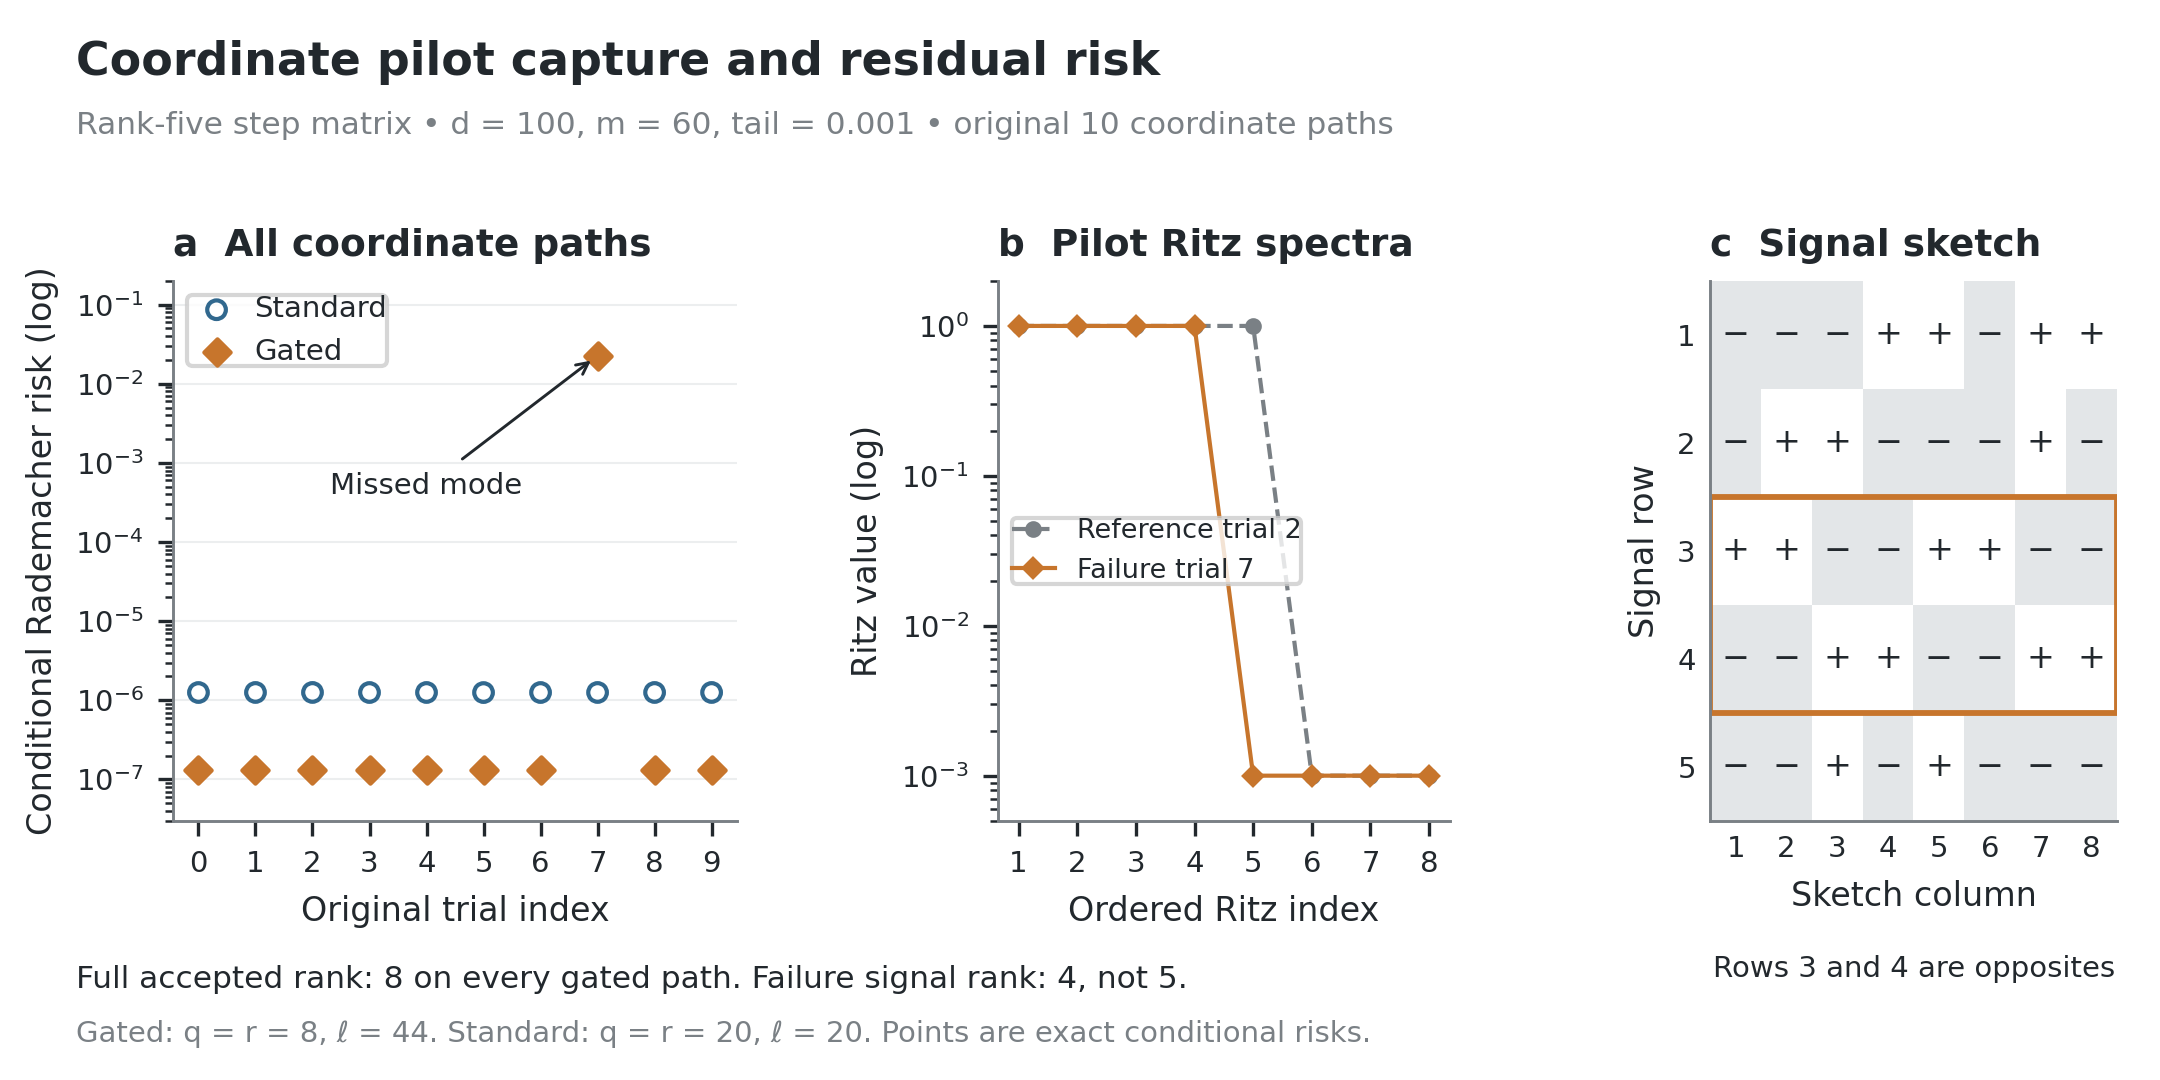
\includegraphics[width=\linewidth]{figures/figure1_capture_failure.png}
\caption[Full rank with incomplete capture]{\textbf{Full rank with incomplete capture.} (a) Exact conditional Rademacher risks for all ten coordinate paths at $d=100$, $m=60$, $k=5$, and $\eta=0.001$. These are not observed squared errors. (b) Pilot Ritz values for the highest-risk path (trial 7) and the median-risk member of the other nine paths (trial 2). (c) The failing $5\times8$ signal sketch has opposite third and fourth rows. Its signal rank is four although the accepted basis rank is eight. The selected spectra illustrate the failure; panel (a) shows the full coordinate sample.}
\label{fig:capture}
\end{figure}
\subsection{Additional gains remain exploratory}\label{exp:E6}
The matrix-free Hessian benchmark used a 4,254-parameter convolutional network on synthetic images. It used the same eight-column pilot rule with logarithmic-gap threshold $1.2$, oversampling parameter two, and no contrast filter. The model has ten outputs, but its labels are only zero and one. The Hessian need not be PSD; Theorems~\ref{thm:T2}--\ref{thm:T3} apply to a symmetric operator, whereas PSD spectral interpretations need additional justification. The floating-point reference trace was approximately 31.581270, obtained using 4,254 reference Hessian--vector products outside the estimator budgets.


{\small
\begin{longtable}{@{}>{\raggedright\arraybackslash}p{0.4224\linewidth}>{\raggedright\arraybackslash}p{0.1936\linewidth}>{\raggedright\arraybackslash}p{0.2640\linewidth}@{}}
\caption{Exploratory synthetic-data Hessian results}\label{tab:auto5}\\
\toprule
Query budget & Standard Hutch++ MSE & Gated MSE \\
\midrule
\endfirsthead
\toprule
Query budget & Standard Hutch++ MSE & Gated MSE \\
\midrule
\endhead
30 & 5.858498 & 5.334005 \\
60 & 1.417330 & 0.841176 \\
90 & 1.006494 & 0.570674 \\
120 & 0.457086 & 0.370210 \\
\bottomrule
\end{longtable}
}
There were 30 trials per method/budget and 480 total across four methods. These point estimates show operator feasibility and gains on this model, not broad ML generalization, a certified safety guarantee, or a wall-clock advantage. The gain cannot be attributed solely to more residual samples because the basis changes too. Sources: Hessian benchmark~\cite{project2026} and recovery audit~\cite{project2026}.


The gate-feature development study~\cite{project2026} contains 23 configurations. Its thresholds were assessed on that same grid; fixed-$q$ empirical minima are noisy grid references, not exact conditional-risk oracles. The later contrast filter was not active in the recovered Haar/Hessian protocols, so those results do not validate that filter.


Earlier YearPredictionMSD and Wiki-Vote studies, including quoted effective ranks, crossover budgets, and reduction factors, remain historical. Those numerical claims have not received source-level reproduction in this consolidation and are not central evidence here. A final external-data claim needs its operator definition, probe law, accounting, replication unit, and uncertainty verified. TurboQuant and leverage-score work remain supporting RandNLA preparation rather than competing main UROP narratives.
